% !TEX program = XeLaTeX
% !TEX encoding = UTF-8
\documentclass[UTF8,nofonts]{ctexart}
\setCJKmainfont[BoldFont=FandolSong-Bold.otf,ItalicFont=FandolKai-Regular.otf]{FandolSong-Regular.otf}
\setCJKsansfont[BoldFont=FandolHei-Bold.otf]{FandolHei-Regular.otf}
\setCJKmonofont{FandolFang-Regular.otf}

\usepackage{url}
\usepackage{cancel}
\usepackage{xspace}
\usepackage{graphicx}
\usepackage{multicol}
\usepackage{subfig}
\usepackage{amsmath}
\usepackage{amssymb}
%\usepackage[a4paper,width=180mm,top=18mm,bottom=22mm,includeheadfoot]{geometry}
\usepackage[a4paper,width=140mm,top=18mm,bottom=22mm,includeheadfoot]{geometry}
\usepackage{booktabs}
\usepackage{array}
\usepackage{verbatim}
\usepackage{caption}
%\usepackage{natbib}
\usepackage{booktabs}
\usepackage{float}
\usepackage{pdflscape}
\usepackage{mathtools}
\usepackage[usenames,dvipsnames]{xcolor}
\usepackage{afterpage}
\usepackage{pgf}
\usepackage{tikz}
\usepackage{dirtree}
\usepackage{amsfonts}
\usepackage{tkz-graph}
\usetikzlibrary{shapes.geometric}%


\title{MTX(Multilateral Token Exchange)Protocol\\一个以太坊代币的多边交易协议}
\author{
    王东 <dong77@gmail.com>
    % \and
    % Haomin Li\\
    % lihaomin@zhongan.io
}

\makeatletter
\def\CTEX@section@format{\Large\bfseries}
\makeatother

\makeatletter
\newenvironment{tablehere}
  {\def\@captype{table}}
  {}

\newenvironment{figurehere}
  {\def\@captype{figure}}
  {}
\makeatother


\begin{document}
\maketitle

\begin{abstract}
本文描述一个开放的,以太坊上ERC20代币间的多边交易协议。通过该协议,可以建立去中心化且无需资产托管的交易所应用。该协议可被视为下一代数字资产交易所的开放标准之一和架构基石。传统交易所可以通过拥抱该协议改进目前交易所的撮合方式,降低用户信任成本和自身运营风险;去中心化应用(dApp)也可也以在智能合约中调用该协议的相关智能合约实现应用内的代币转换。

\end{abstract}

\section{背景介绍\label{sec:background}}

区块链作为比特币的底层技术,本质上是去中心化无信任环境中的存在性共识。存在性可应用于各种不同的数据,如股权,版权,使用权等。尽管联盟链和企业私有链中共识数据的类别正在变得越来越多样化,但这些数据的价值却有着明确的边界限制 - 只限于联盟成员间和企业内部。我们认为区块链的价值网络属性在公有链中才会的到更好的体现。根据coinmarketcap.com的统计,截止本文成稿时间,区块链上代币总市值已经超过790亿美元,以太坊区块链上承载的代币市值超过170亿美元。

区块链对各个行业都将有着深远的影响,尤其是金融领域。我们相信基于区块链的新金融会有一个明显趋势,即资产代币化(Tokenization):一方面链下资产的使用权,所有权,分红权等相关权益产通过抵押会被发行到区块链上,另一方面区块链上资产也会进行跨链发行。资产代币化的重要目标之一就是低成本,全球化,全天候的高流动性,而流动性则主要通过交易机制和交易所得以实现。

在现阶段,提供主要流动性的交易所都有非常类似的模式:交易所要求用户将法币或者代币充值到交易所的银行或区块链账户中,然后交易所在自己中心服务器的虚拟账户系统中为用户进行IOU记账。用户实际交易的是这些IOU。为了将IOU兑换成法币或区块链代币,用户需要向交易所提出提现请求,提现成功后,才算真正交易完成。在这个过程中,交易所替用户安全保管资产的能力是用户最大的风险;同时用户还需担心交易所运营者的商业道德问题,比如挪用资金造成资不抵债等。2014年2月当时世界最大规模的比特币交易所运营商Mt.Gox的85万个比特币被盗一空,公司向日本东京地方法院申请破产保护。该公司的用户至今仍在等待其返还尚未被盗的少量比特币。随着调查的不断进行Mt.Gox被曝出所谓的比特币被盗其实是监守自盗。85万个“被偷窃”的比特币中,实际上因外部盗窃失踪的仅为7000个。而包括比特币存钱罐和ShapeShift在内的平台被盗事件也被曝出涉及内部人士。2016年8月最大的美元比特币交易平台香港的Bitfinex由于网站出现安全漏洞,导致用户持有的比特币被盗,被盗的比特币共119756枚,总价值约为6500万美元。随后该公司决定由所有用户共同分担损失以避免其破产。交易所缺失的资产保管能力和监守自盗的败坏的商业道德,一方面反映出比特币在各个国家监管政策的缺失与漏洞,另一方面也证实中心化交易所模式的固有风险。

基于区块链的去中心化交易机制就是为了彻底解决上述问题。去中心化交易的核心优势之一是避免任何资产被托管,因此资产就不存在被盗的可能性,这会极大降低用户对交易所的信任成本;这种交易机制的另一个优势是没有地缘和时间限制,以及极高的透明性和可追溯性。这些特点会促使交易整体具有更大的流动性和更小的买卖价差。

\section{相关工作\label{sec:existingworks}}
我们希望通过采用区块链\cite{nakamoto2008bitcoin,swan2015blockchain}和去中心化存储技术,实现一种基于银行联盟的新型支付解决方案。该方案需要实现的目标包括:

[几个段落:介绍早期区块链上交易所的尝试,特别是Ripple的机制。


[几个段落:介绍一些automatic market maker算法,包括Bancor协议,{Price Evolution in a Continuous Double Auction Prediction Market With a Scoring-Rule Based Market Maker}, {Hanson, R. 2003a. Book orders for market scoring rules. George Manson University.}]

[一个稍长的段落:介绍0x协议,指明其缺点,比如:1)taker负责匹配订单,要求taker在线,撮合实时性差因此撮合价格无法及时优化,2)实际就是简单的OTC方式,没法实现复杂订单的撮合,3)交易所之间没有明确的竞争激励机制,4)没有考虑旷工的利益。]

我们受0x协议和闪电网络的启发,提出一个以太坊上ERC20代币间交易协议。通过该协议,代币持有者可以通过数字签名授权指定的一个或多个交易所帮助自己撮合订单,并将该订单在链下广播给交易所;交易所会使用与MTX智能合约中相同的逻辑对多个订单进行匹配,通过数字签名生成区块链交易,并负责将交易广播到以太坊网络,并通过触发智能合约实时完成代币在相关交易方间的清算和转账。

\section{MTX协议\label{sec:protocol}}

\begin{center}
\begin{figurehere}
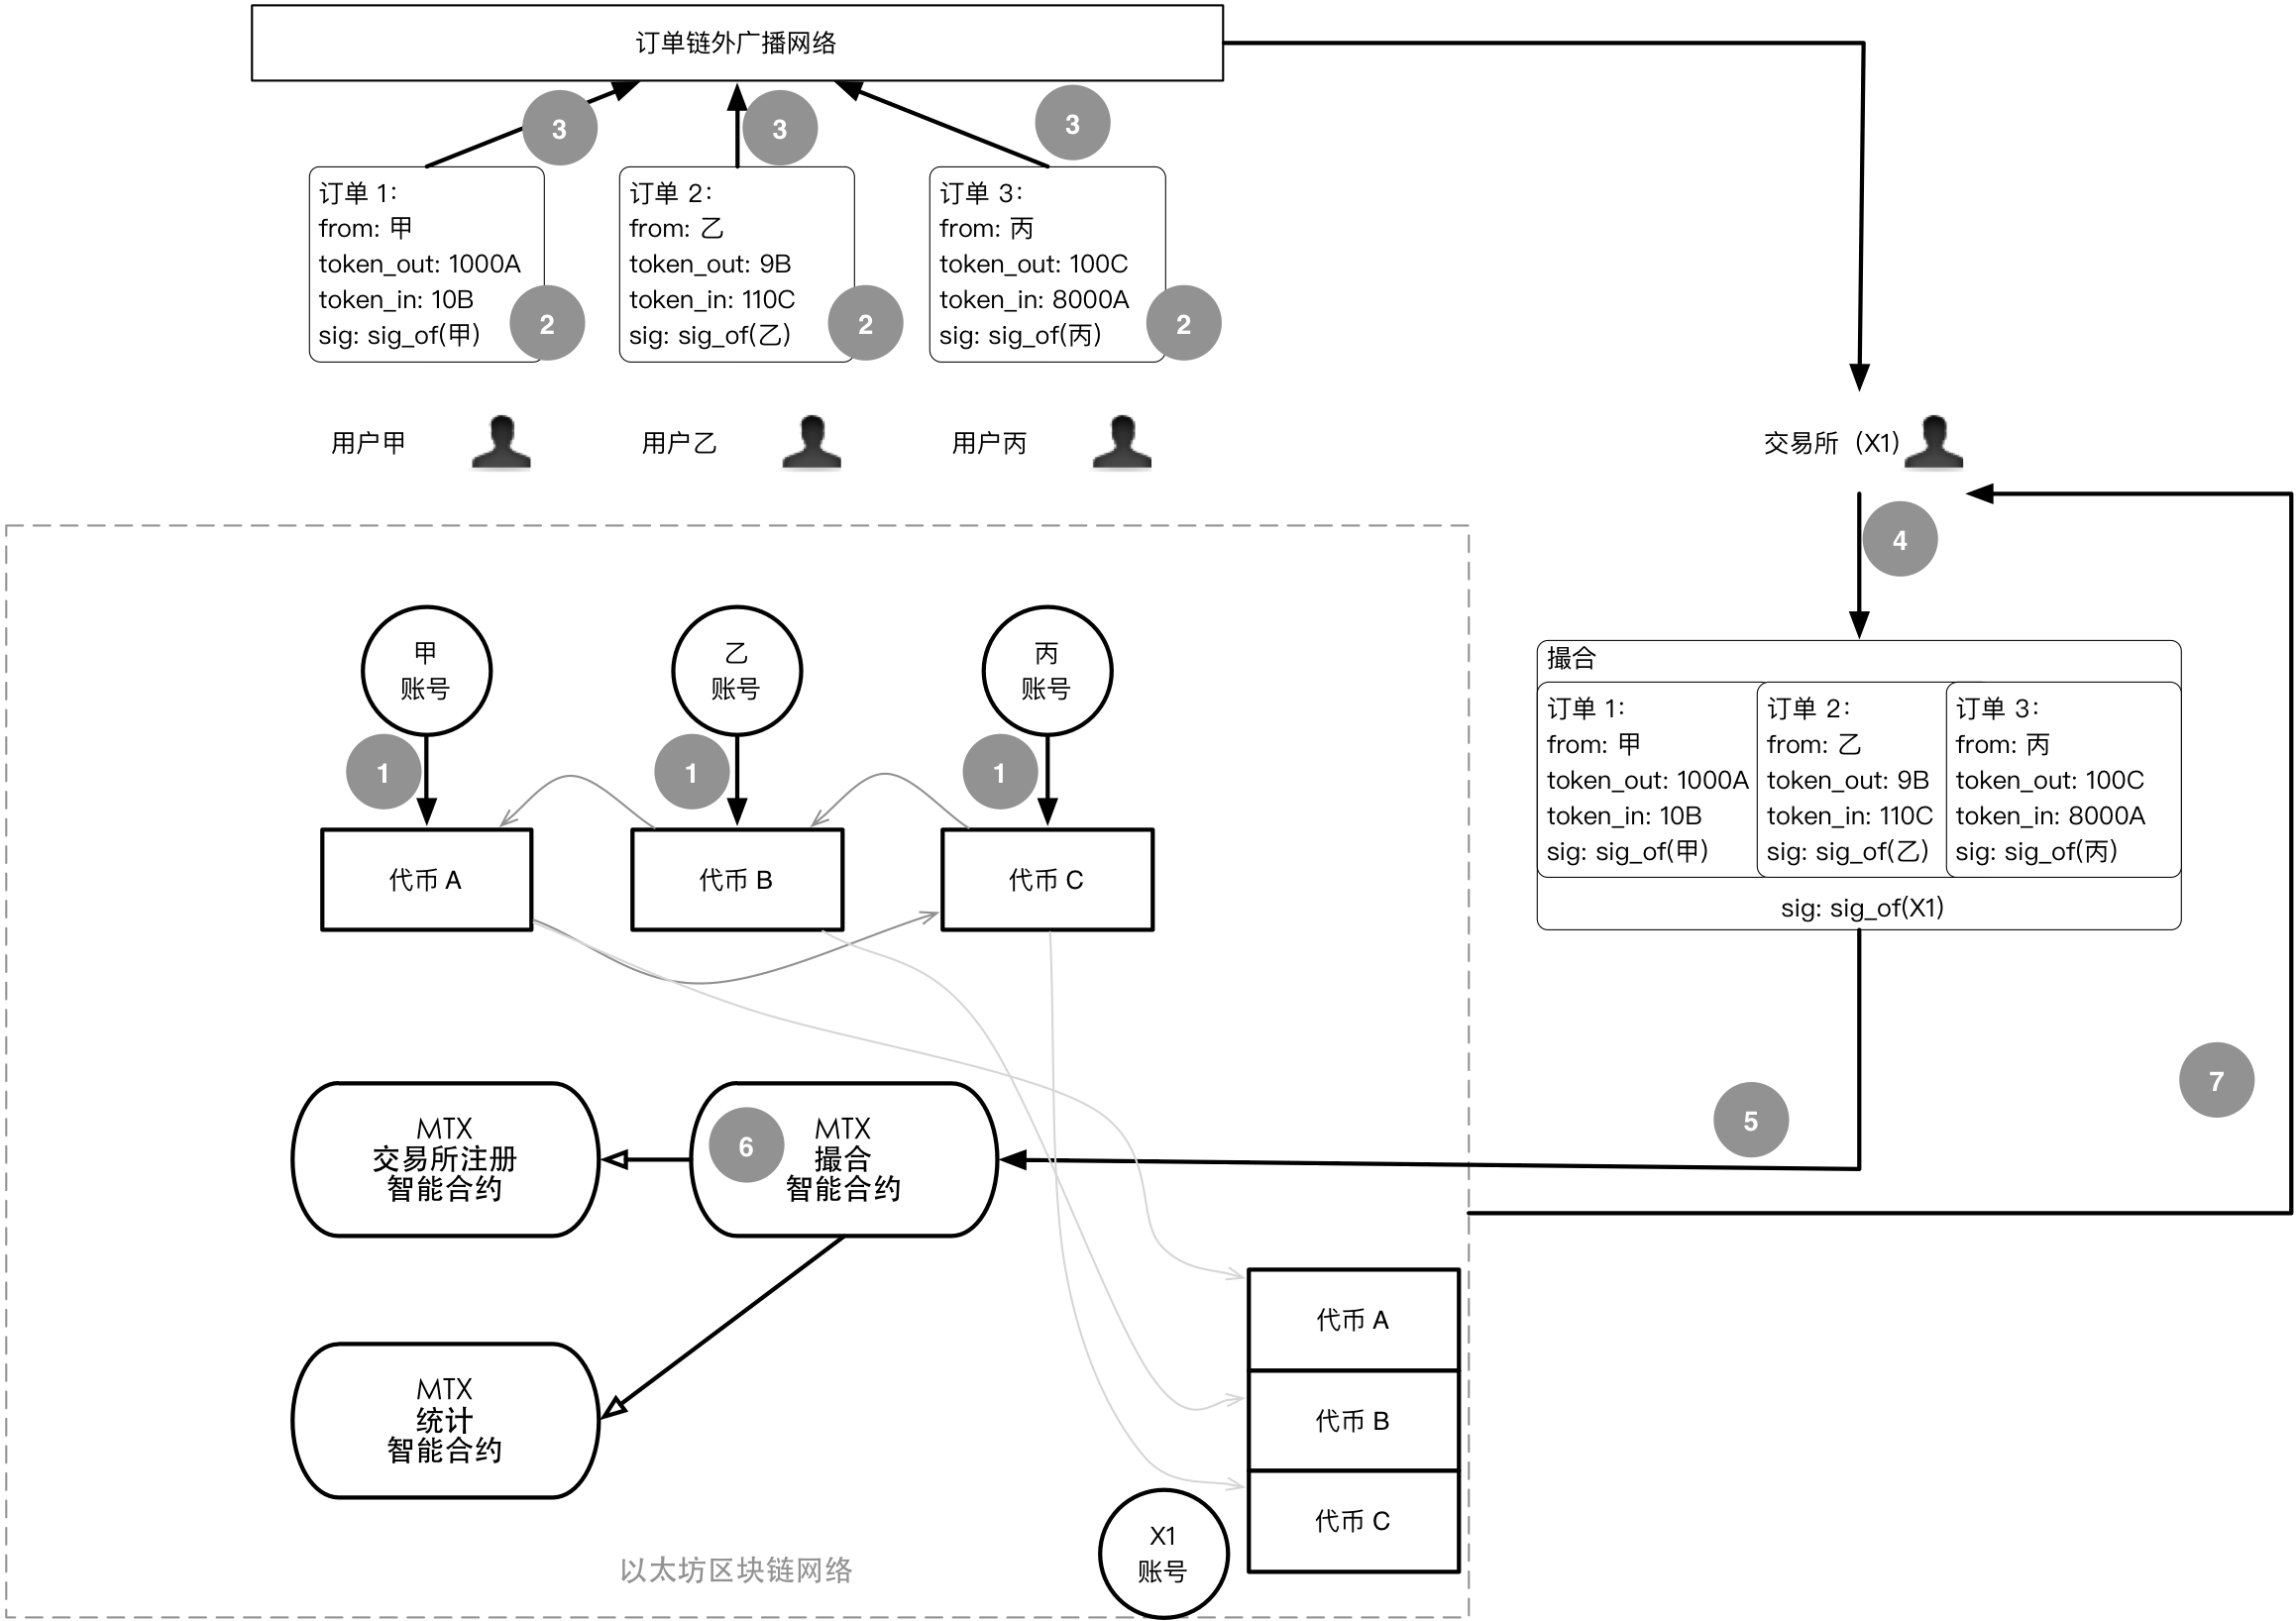
\includegraphics[height=10cm]{images/mtx-protocol.png}
\caption{一个三边交易通过MTX协议撮合的示例}
\label{fig:mtxprotocol}
\end{figurehere}
\end{center}



\subsection{定价机制\label{sec:pricediscovery}}

[段落:讲讲中心和交易所的定价模型,以及为什么不适合于去中心化交易所 double action vs taker maker]

[段落,讲讲我们的定价模型:我们属于double auction模型,采用中间级成交,同时讲讲交易所收费]

[段落:价格发现机制的理论证明]

[段落:成绩额度的计算]

[段落:交易所费用的计算]

\subsection{数据格式\label{sec:dataformat}}

订单格式,撮合格式。

\subsection{智能合约\label{sec:smartcontract}}


[段落:讲讲订单状态]

[段落:部分成交和取消订单]

[段落:讲讲撮合成功条件]


[段落:代币名字注册合约]

[段落:交易所注册合约]

[段落:交易所统计合约]

[段落:token兑换率统计合约]


\subsection{交易所\label{sec:exchange}}


[段落:价值,收入,相互竞争,交易所时间和利润的平衡,旷工对撮合的选择和利益]

[段落:交易所评分]

[段落:交易所如何实现短期利润最大化]

[段落:交易所的信用积累]

[段落:交易所的初创成本]


\section{协议代币\label{sec:exchangetoken}}

[段落:代币用于支付交易费,更节约成本]

[段落:交易所购买代币进行注册的抵押]

[段落:协议代币也是ERC20,可以同样方式交易,因此生态是个完整闭环]

\section{鸣谢\label{sec:acknowledgement}}

\bibliography{whitepaper}
\bibliographystyle{acm}

\end{document} 